%%Este capítulo debe ser el primer tema técnico a tratar,
%%debido a que mi tema se trata al modelado de objetos 
%%y de servicios de comunicación (al final los servicios
%%de comunicación se modelan como objetos via xml)
%%y también la utilización de interfaces da una buena base
%%para entender las capas del modelo OSI: las interfaces
%%que posee cada capa para comunicarse con las otras
%%(servicios) son muy bien compreendidas una vez
%%tratada el tema de interfaces de OOP. Al final, 
%%este tema de interfaces es 
%%abstracción, tratada en ingeniería de software. Por 
%%ello, es un buen punto empezar desde aquí.

\chapter{Object-oriented programming}

\section{Introduction}

The IEC 61850 information model 
is classified as a  
\glsentrytext{O-O} system. Is necessary 
to have a clear understanding of \gls{O-O} technology
to dive into IEC 61850 object modelling. 
For this reason this chapter describes 
the \gls{O-O} technology
on which the IEC 61850 information model 
has been standarized\todo[inline]{No se si esta 
bien escrita la palabra standarized}. 

The chapter does not describe all the \gls{O-O} principles, 
just \todo{�trans:just focuses or focuses just?} focuses 
on the neccesary
background to understand the IEC 61850 
information model. 
The sections which follow will define the 
background which the IEC 61850 
object oriented information system 
was constructed, both formally 
and through examples.
\todo[inline]{debo agregar las abreviaciones de O-O
a mi glossaries package}
A detailed description of the \gls{O-O} fundamentals  
and reference materials are provided. To achieve a 
robust concepts comprehension a practical 
implementation with the%the Unified Modeling Language 
\gls{UML} 
\todo{agregar al glossaries} 
\cite{UML2:2009} 
and Java \cite{Java:specification} are provided. 
This chapter is very
practical in the sense that uses language programmings to model 
very carefully selected models  
used by the IEC 61850 standard, 
(but not explaining explicitly nothing 
about the standard yet!).
This chapter is destined 
for electrical engineers and professionals of 
related areas readers which the \gls{O-O} software construction 
is not part of the curriculum. For this reason, 
the practical examples uses electricity area 
elements. The readers with a strong knowledge 
of programming could skip this
chapter \todo[inline, color=blue!50!red!50]{
	deber\'ia agregar esta ultima frase?:
	\emph{The readers with a strong knowledge 
	of programming could skip this
	chapter}
}




\todo[inline]{En este cap�tulo voy a agregar 
los graficos a continuacion:

(los ejemplos que voy usando son con estas clases)}


\begin{figure}
  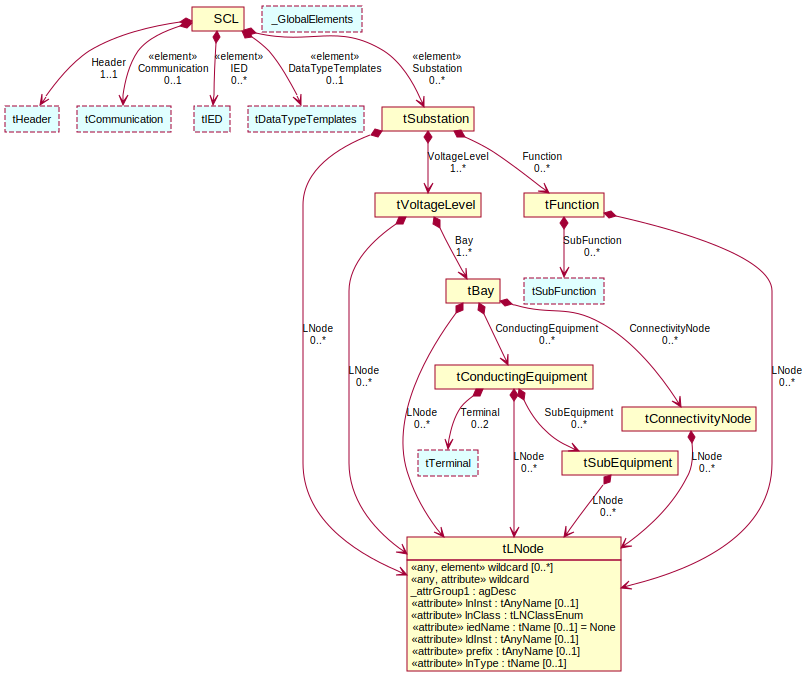
\includegraphics[width=1.0\textwidth]{chapters/ch-oop/figures/LogicalNodeAllocationStructure}
  \caption{Logical Node and their role at the substation level}
  \label{fig:LogicalNodeAllocationStructure}
\end{figure}

\begin{landscape}
	\begin{figure}	
	  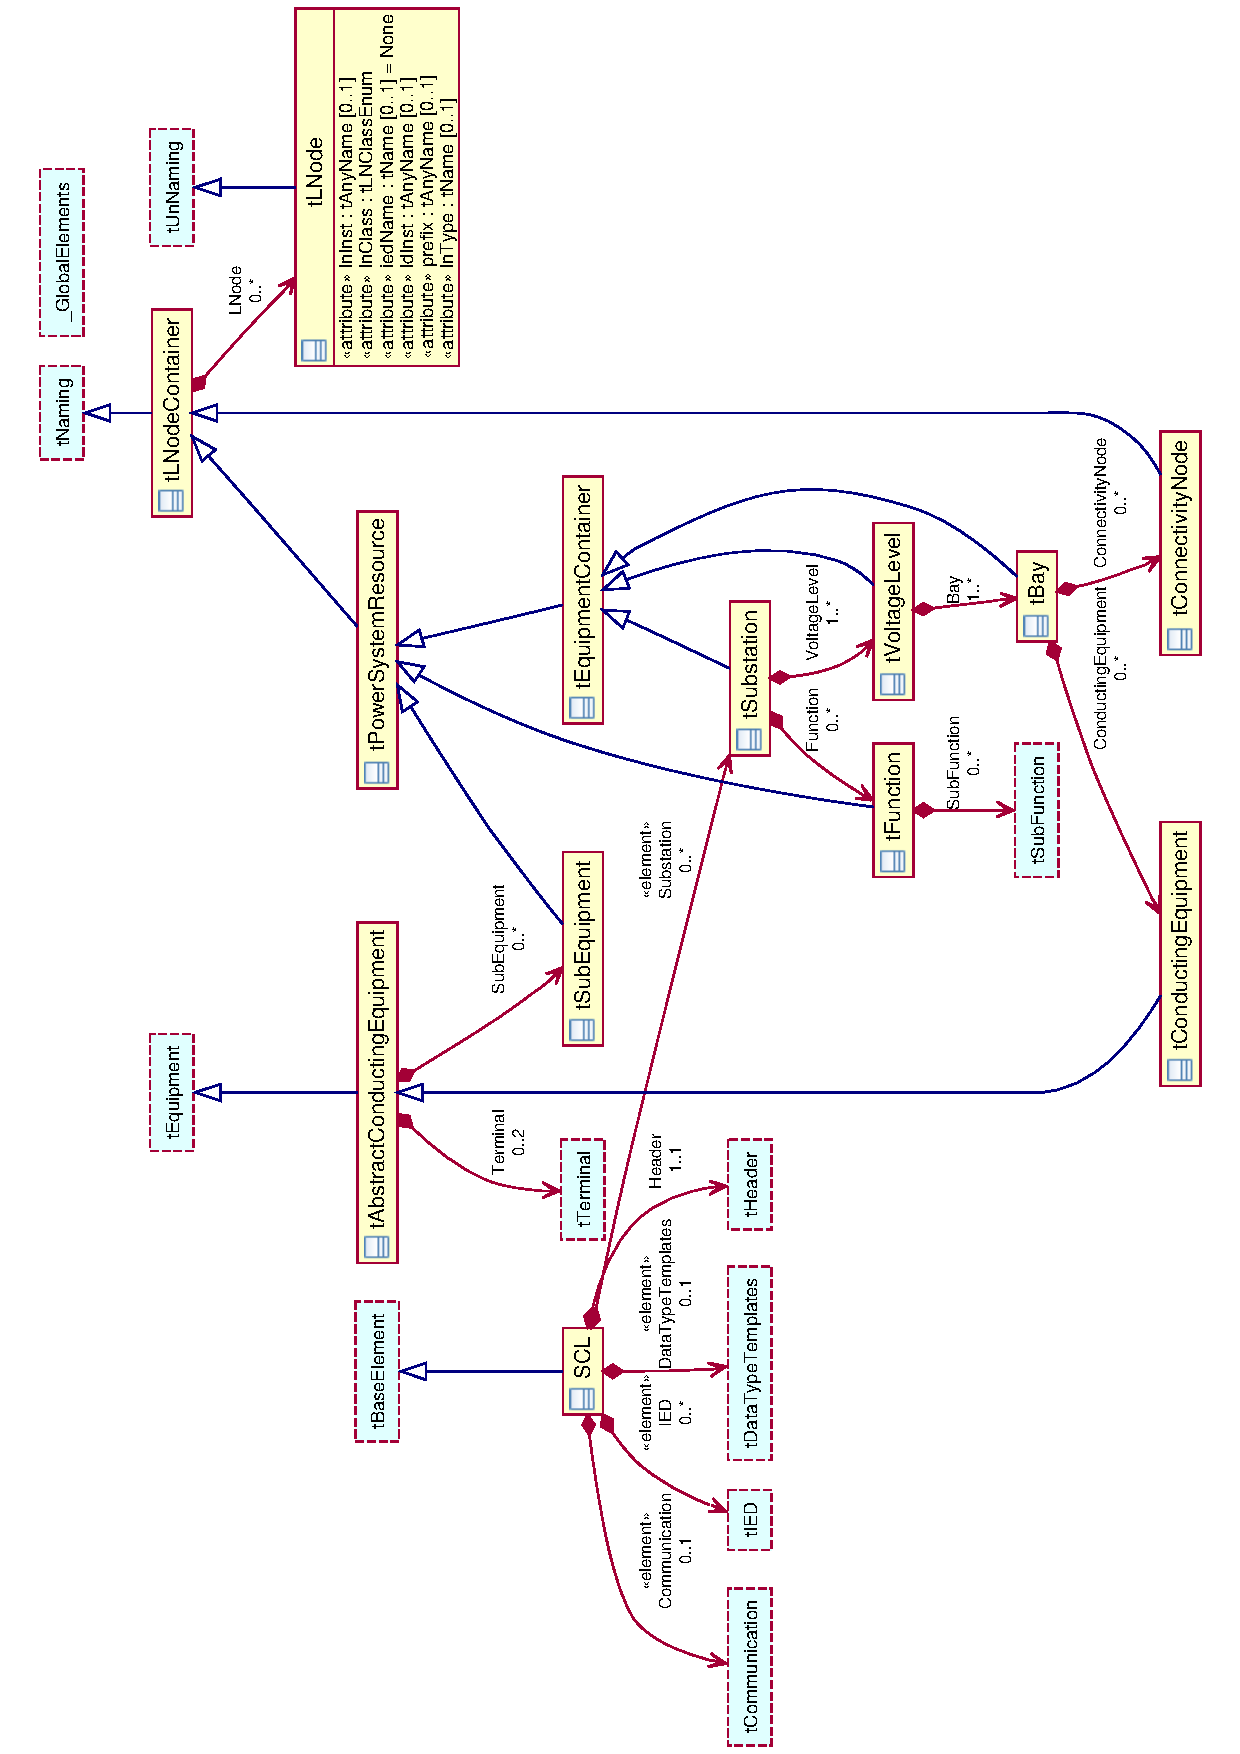
\includegraphics[angle=-90, width=1.0\linewidth]{chapters/ch-oop/figures/LogicalNodeAllocationStructure_with_heritance}
	  \caption{Logical Node and their role at the substation level, depicted with
	  the heritance details}
	  \label{fig:LogicalNodeAllocationStructure_with_heritance}
	\end{figure}
\end{landscape}
	
\section{Basics of object-oriented programming}

\subsection{Introduction to object-oriented programming}

%TODO: citar
%esta parte fue obtenida del libro de adobe, del cap 5. 
Object-oriented programming (OOP) is a way of organizing the code 
in a program by grouping it into objects-individual elements that include 
information (data values) and functionality. Using an 
object-oriented approach to organizing a program allows 
you to group particular pieces of information (for 
example, a automation function or a current value) together with 
common functionality or actions associated with that 
information (such as ``switchgear actuation'' or 
``voltage measurement''). These items are combined into a single 
item, an object (for example, an 
\todo[size=\tiny]{cambiar por un ejemplo el\'ectrico}
``Album'' or ``MusicTrack''). Being 
able to bundle these values and functions together provides several 
benefits, including only needing to keep track of a single 
variable rather than multiple ones, organizing related 
functionality together, and being able to structure 
programs in ways that more closely match the real world.  


\subsection{Common object-oriented programming tasks}

%Aca va la pagina 99 de actionscript programming.
In practice, 
%citar las prácticas comunes
\begin{itemize}
	\item Defining classes
	\item Creating properties, methods, and get and set accessors (accessor
	methods) 
	\item Controlling access to classes, properties, methods, and accessors
	\item Creating static properties and methods
	\item Creating enumeration-like structures
	\item Defining and using interfaces
	\item Working with inheritance, including overriding class elements 
\end{itemize}



\section{Classes}

A class is a static 
%off-line \todo{es realmente off-line?}
template from which objects are 
created. Classes are used 
to classify objects thanks 
that its defines 
common operations 
and a data structure, 
and the types of 
datas that the object can 
store.\\


%Codigo fuente
%C:\Documents and Settings\DELL\Mis
%documentos\tesismayo\tesismayo\thesis\chapters\ch-oop\source\java\src\HelloWorld.java
%\lstinputlisting[label=samplecode,caption=A sample]{sourceCode/HelloWorld.java}
%chapters\ch-oop\source\java\src\HelloWorld.java
\lstinputlisting[label=codeClass,
caption=Class in Java]{chapters/ch-oop/source/java/src/SERVER_v1.java}

%%TODO: cite adobe book

\subsection{Attributes}
\todo[inline]{completar esta parte}
	\lstinputlisting[label=codeAttributes,
	caption=Class with attributes in Java]
	{chapters/ch-oop/source/java/src/SERVER_v2.java}



\subsection{Methods}
Methods are functions that are part of a class 
definition. Once an instance of the class is created, 
a method is bound to that instance.\\
	\lstinputlisting[label=codeMethod,
	caption=Class with attributes and methods in Java]
	{chapters/ch-oop/source/java/src/SERVER_v3.java}



	\subsubsection{Get and set accessor methods}
	Get and set accessor functions, also called getters 
	and setters, allow you to adhere to the programming principles of 
	information hiding and encapsulation while providing an 
	easy-to-use programming interface for the classes that you 
	create. Get and set functions allow you to keep your class 
	properties private to the class, but allow users of your class 
	to access those properties as if they were accessing a 
	class variable instead of calling a class method. 
	The advantage of this approach is that you can avoid 
	having two public-facing functions for each property 
	that allows both read and write access. \\

		\lstinputlisting[label=codeMethod,
		caption=Class with attributes, methods, getters and setters in Java]
		{chapters/ch-oop/source/java/src/SERVER_v4.java}
	
	
	\subsubsection{Constructor methods}
	Constructor methods, sometimes simply called constructors, 
	are functions that share the same name as the class in 
	which they are defined. Any code that you include in 
	a constructor method is executed whenever an instance of the 
	class is created with the  new  keyword. \\

		\lstinputlisting[label=codeMethod,
		caption=Class with attributes, methods, 
		getters, setters and constructors in
		Java] {chapters/ch-oop/source/java/src/SERVER_v5.java}

	
\section{Intefaces}

%\input{chapters/ch-oop/blah blah blah}
